\documentclass{article}

% Recommended, but optional, packages for figures and better typesetting:
\usepackage{microtype}
\usepackage{graphicx}
\usepackage{subfigure}
\usepackage{booktabs} % for professional tables

\usepackage{hyperref}
\usepackage{amsmath}
\usepackage{amssymb}

\newcommand{\theHalgorithm}{\arabic{algorithm}}

\usepackage[accepted]{icml2018}

\icmltitlerunning{Online Recommendation via Particle Thompson Sampling}

\begin{document}

\twocolumn[
\icmltitle{Online Recommendation via Particle Thompson Sampling}
\begin{icmlauthorlist}
\icmlauthor{Michael Alvarino}{equal}
\icmlauthor{Bharat Srikishan}{equal}
\icmlauthor{Colby Wise}{equal}
\end{icmlauthorlist}
\icmlaffiliation{equal}{Columbia University}
\vskip 0.3in
]

\begin{abstract}
    Within the field of recommender systems various forms of collaborative filtering are often used to estimate how users will rate items. One of the most popular methods used when contextual information is not available is Probabilistic Matrix Factorization (PMF). This core method is capable of scaling with a large number of observations and performs well even when restricted to sparse datasets. Unfortunately PMF is limited to offline predictions for a fixed set of users and items. First, we present a fast online recommendation system using PMF, Thompson sampling, and particle filtering to provide cold start movie recommendations to users. Then we provide a method for evaluating algorithm performance on users with high drift in preferences. Lastly, we examine the effect of different particle sampling methods on particle degeneracy.
\end{abstract}

\section{Introduction}
PMF is the most common collaborative filtering method for recommendation systems. While it does provide useful recommendations for users it also requires a-priori knowledge of the set of users and items. Real world use cases must provide recommendations for users that have no previous history (cold start users). 

Online learning methods are designed to accept new users or items over time without sacrificing the efficiency or accuracy of the algorithm. In Efficient Thompson Sampling for Online Matrix Factorization Recommendation \cite{kawale2015efficient} (ETSOMF) an online algorithm is proposed, but is subject to degeneracy, a common problem in particle filtering methods.

A particle filtering algorithm is said be degenerate when, after only a few iterations, all but one particle has negligible weights. We propose several different particle resampling methods which combat the degeneracy problem and compare their performance on the MovieLens 100k Dataset.

\section{Model}

\subsection{Probabilistic Matrix Factorization}
Offline PMF computes a low rank factorization of a ratings matrix $R$ where $R = UV^\top$ for $U \in \mathbb{R}^{n \times k}$
and $V \in \mathbb{R}^{m \times k}$. $U$ and $V$ are user and item latent matrices and $K$ is small, for most of our experiments $K$ was less than $10$.

The PMF model assigns a Normal prior with zero mean and $K$ dimensional user-specific variance, $\sigma_u^2 I_K$, to the user latent matrix $U$ and a similar distribution to the item latent matrix $V$. Each rating $r_{i,j}$ is then assigned a Normal distribution centered on $U_iV_j^T$ with rating variance $\sigma^2$.

\begin{center}
$U_i \sim \mathcal{N}(0, \sigma_u^2 I_K)$ \\
$V_i \sim \mathcal{N}(0, \sigma_v^2 I_K)$ \\
$r_{ij} | U, V \sim \mathcal{N}(U_i^\top V_j, \sigma^2)$
\end{center}

This linear Gaussian model has an analytically solvable conditional posterior, but in order to support online inference we use a particle filtering method as described in ETSOMF.

\subsection{Particle Filtering}
Particle Filtering is a well-known Sequential Monte Carlo method for performing inference in state of a systems where the system evolves over time based on information from noisy measurements. Sequential importance sampling ($SIS$) is a approximate Monte Carlo particle filtering method for analytically intractable systems. The goal of SIS is to approximate a posterior distribution with a weighted set of "samples" known as particles. The key idea is to update particles and their weights with new information at each step to better approximate the target posterior.  

Let $\{X_{0:k}^i, w_k^i\}_1^N$ denote N random measures representative of the posterior of a system, $p(x_{0:k}| z_{1:k})$. Then, we can approximate the true posterior of this system by the following

\begin{center}
    $p(x_{0:k}| z_{1:k}) \approx \Sigma_{i=1}^{N}w^i_k \delta(x_{0:k} - x^i_{0:k})$ \\
    \text{where }  $\Sigma_i w_k^i = 1$ \\
\end{center}

Then, using sequential importance sampling, we can derive update equations for the weight associated with each particle as described in \cite{arulampalam2002tutorial}.

\subsection{Resampling}
A common problem with particle filtering methods such as SIS is particle $degeneracy$. Particle degeneracy is the tendency for only a few particle weights to have significant mass while all other weights drift toward zero as particles are successively updated.

Resampling is a common way to deal with the degeneracy problem. During resampling we draw a new set of N particles with replacement from the current particles based on the normalized weights of the current particle set. The advantage of this method is that it allows us to carry forward particles with high probability mass areas. The down-side of resampling is called $sample$ $impoverishment$. Sample impoverishment is when particles with large weights are sampled more frequently than low weight particles leading to a decrease in diversity of particles. It is common for the number of particles to collapse into a single particle which can negatively effect the quality of the approximation.

The original authors of ETSOMF saw degeneracy as a significant problem while training their algorithm. Our contribution is the analysis of new resampling methods for combating degeneracy. Specifically, we examine three primary resampling techniques, multinomial, stratified, and systematic resampling.

\subsubsection{Multinomial Resampling}
In multinomial resampling the particles are sampled from a multinomial distribution whose parameters are directly defined by the normalized, updated, weights of each particle \cite{douc2005comparison}.

\subsubsection{Stratified Resampling}
Stratified resampling breaks the interval into $n$ disjoint sets $(0, 1/n], ... , (\{n - 1\} / n, 1]$ and draws independently from the uniform distribution $U((\{i - 1\}/n, i/n])$ where $i$ is the $i$-ith sample \cite{douc2005comparison}.

\subsubsection{Systematic Resampling}
Systematic resampling deterministically links variables drawn in sub-intervals during stratified sampling. It does so by setting $U^i = (i-1)/n + U$, where $U$ is drawn from $U((0, 1/n])$.

$U$s generated via systematic resampling are known within the particle sampling literature as empirically good and computationally simple \cite{douc2005comparison}

\subsection{Particle Thompson Sampling}
We take advantage of the graphical structure of our probabilistic model to derive an efficient Rao-Blackwellized particle filter which maintains an estimate of the posterior over time. Additionally, we use Thompson sampling to choose particles and balance exploration with exploitation of our current posterior estimate.

Each particle stores parameters $U, V, \sigma_U, \sigma_V$ and we for each update sample $U_{i_t}|V, \sigma_U$
followed by $V_{j_t}|U, \sigma_v$:
\begin{center}
$P(U_i | V, R^o, \sigma, \sigma_U) = P(U_i | V_{rts(i)}, R^o_{i, rts(i)}, \sigma_U, \sigma)$ \\
$= \mathcal{N}(U_i | \mu^u_i, (\Lambda_i^u)^{-1})$ \\
\ \newline
\text{where } $\mu_i^u = \frac{1}{\sigma^2}(\Lambda_i^u)^{-1})\zeta_i^u$ \\
\ \newline
$\Lambda_i^u = \frac{1}{\sigma^2} \sum_{j \in rts(i)} V_j V_j^{\top} + \frac{1}{\sigma_u^2}I_K$ \\
\ \newline
$\zeta_i^u = \sum_{j \in rts(i)} r_{ij}^o V_j$
\end{center}


Here $R^o$ are the observed ratings and $rts(i)$ is the set of items rated by user $i$. The update for our sample of $V_j$ mirrors this update.


\section{Experiments}

\subsection{Data}
We ran our experiments on the MovieLens 100k dataset. We only used the rating data for our
online recommendations, however we used the genre data in our evaluation of user preference
drift. We subtracted the mean rating from the data to center ratings at 0.

This dataset has 943 users, 1683 movies, and 100,000 ratings.

\section{Results}

\subsection{MSE}
\begin{figure}[ht]

\begin{center}
\centerline{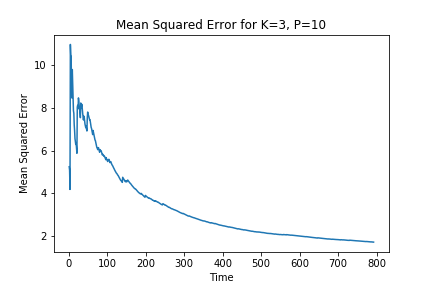
\includegraphics[width=\columnwidth]{TrainMSE}}
\caption{Training set mean squared error over time for K = 3 and 10 particles.}
\label{TrainMSE}
\end{center}

\vskip -0.2in
\end{figure}

We first examine mean squared error on the training set. As we see in Figure \ref{TrainMSE}, it decreases
over time as expected. The final MSE in this case is 1.721.

\begin{table}[ht]
\caption{Mean squared error statistics on the test set for various choices of K
(latent dimensionality) and P (number of particles)}
\label{sample-table}
\vskip 0.15in
\begin{center}
\begin{small}
\begin{sc}
\begin{tabular}{lcccc}
\toprule
(K, P) & Mean & Std Dev & Min & Max \\
\midrule
(2, 2)  & 2.924 & 0.355 & 2.512 & 3.585 \\
(2, 5)  & 2.981 & 0.387 & 2.552 & 3.711 \\
(3, 5)  & 2.540 & 0.182 & 2.408 & 2.900 \\
(3, 10) & 2.838 & 0.507 & 2.326 & 3.639 \\
(5, 2)  & 2.329 & 0.086 & 2.199 & 2.441 \\
(5, 10) & 2.367 & 0.088 & 2.251 & 2.519 \\
(5, 20) & 2.357 & 0.062 & 2.250 & 2.413 \\
\bottomrule
\end{tabular}
\end{sc}
\end{small}
\end{center}
\vskip -0.1in
\end{table}

\subsection{Cumulative Take Rate}

\subsection{Hyperparameter Cross Validation}

\subsection{User Preference Drift}

\section{Conclusion}

\nocite{kawale2015efficient}
\nocite{wang2017online}
\nocite{zhao2013interactive}
\nocite{cherkassky2013sequential}
\nocite{arulampalam2002tutorial}
\nocite{douc2005comparison}

\bibliographystyle{icml2018}
\bibliography{report}

\end{document}
